% Options for packages loaded elsewhere
\PassOptionsToPackage{unicode}{hyperref}
\PassOptionsToPackage{hyphens}{url}
%
\documentclass[
]{book}
\title{EEBE stats}
\author{Alejandro Caceres}
\date{2023-09-04}

\usepackage{amsmath,amssymb}
\usepackage{lmodern}
\usepackage{iftex}
\ifPDFTeX
  \usepackage[T1]{fontenc}
  \usepackage[utf8]{inputenc}
  \usepackage{textcomp} % provide euro and other symbols
\else % if luatex or xetex
  \usepackage{unicode-math}
  \defaultfontfeatures{Scale=MatchLowercase}
  \defaultfontfeatures[\rmfamily]{Ligatures=TeX,Scale=1}
\fi
% Use upquote if available, for straight quotes in verbatim environments
\IfFileExists{upquote.sty}{\usepackage{upquote}}{}
\IfFileExists{microtype.sty}{% use microtype if available
  \usepackage[]{microtype}
  \UseMicrotypeSet[protrusion]{basicmath} % disable protrusion for tt fonts
}{}
\makeatletter
\@ifundefined{KOMAClassName}{% if non-KOMA class
  \IfFileExists{parskip.sty}{%
    \usepackage{parskip}
  }{% else
    \setlength{\parindent}{0pt}
    \setlength{\parskip}{6pt plus 2pt minus 1pt}}
}{% if KOMA class
  \KOMAoptions{parskip=half}}
\makeatother
\usepackage{xcolor}
\IfFileExists{xurl.sty}{\usepackage{xurl}}{} % add URL line breaks if available
\IfFileExists{bookmark.sty}{\usepackage{bookmark}}{\usepackage{hyperref}}
\hypersetup{
  pdftitle={EEBE stats},
  pdfauthor={Alejandro Caceres},
  hidelinks,
  pdfcreator={LaTeX via pandoc}}
\urlstyle{same} % disable monospaced font for URLs
\usepackage{longtable,booktabs,array}
\usepackage{calc} % for calculating minipage widths
% Correct order of tables after \paragraph or \subparagraph
\usepackage{etoolbox}
\makeatletter
\patchcmd\longtable{\par}{\if@noskipsec\mbox{}\fi\par}{}{}
\makeatother
% Allow footnotes in longtable head/foot
\IfFileExists{footnotehyper.sty}{\usepackage{footnotehyper}}{\usepackage{footnote}}
\makesavenoteenv{longtable}
\usepackage{graphicx}
\makeatletter
\def\maxwidth{\ifdim\Gin@nat@width>\linewidth\linewidth\else\Gin@nat@width\fi}
\def\maxheight{\ifdim\Gin@nat@height>\textheight\textheight\else\Gin@nat@height\fi}
\makeatother
% Scale images if necessary, so that they will not overflow the page
% margins by default, and it is still possible to overwrite the defaults
% using explicit options in \includegraphics[width, height, ...]{}
\setkeys{Gin}{width=\maxwidth,height=\maxheight,keepaspectratio}
% Set default figure placement to htbp
\makeatletter
\def\fps@figure{htbp}
\makeatother
\setlength{\emergencystretch}{3em} % prevent overfull lines
\providecommand{\tightlist}{%
  \setlength{\itemsep}{0pt}\setlength{\parskip}{0pt}}
\setcounter{secnumdepth}{5}
\usepackage{booktabs}
\ifLuaTeX
  \usepackage{selnolig}  % disable illegal ligatures
\fi
\usepackage[]{natbib}
\bibliographystyle{plainnat}

\begin{document}
\maketitle

{
\setcounter{tocdepth}{1}
\tableofcontents
}
\hypertarget{objective}{%
\chapter{Objective}\label{objective}}

This is the introduction course to the statistics of the EEBE (UPC).

Statistics is a \textbf{language} that allows you to face new problems, on which we have no solution, and where the \textbf{randomness} plays a crucial role.

In this course we will discuss the \textbf{fundamental concepts} of statistics.

\begin{itemize}
\item
  3 hours of \textbf{Theory} per week: we will explain the concepts, we will exercise.
\item
  6 hours of \textbf{Individual study} per week: notes of course notes and resources in Athena.
\item
  2 hours of problem solving with \textbf{R}: face-to-face sessions (practices).
\end{itemize}

Exam dates and additional study material can be found in \textbf{ATENEA metacurso}:

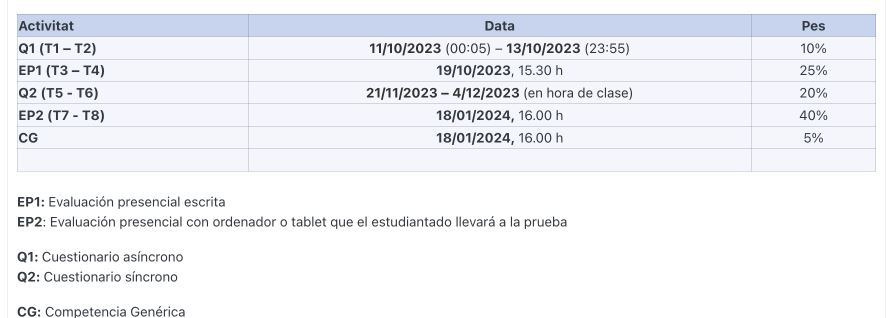
\includegraphics{./figures/notas.JPG}

Evaluation objectives:

\textbf{Q1} (10\%): Test in computer Duration 2h on the indicated dates.

\begin{enumerate}
\def\labelenumi{\alph{enumi}.}
\tightlist
\item
  Basic command knowledge (practices)
\item
  Ability to calculate descriptive statistics and graphics, in specific situations (theory/practice)
\item
  Knowledge about linear regression (practices)
\end{enumerate}

\textbf{EP1} (25\%): Written test (2-3 problems)

\begin{enumerate}
\def\labelenumi{\alph{enumi}.}
\tightlist
\item
  Capacity to interpret statements in probability formulas (theory).
\item
  Knowledge of the basic tools to solve problems of joint probability and conditional probability (theory).
\item
  Mathematical knowledge of probability functions to calculate its basic properties (theory).
\end{enumerate}

\textbf{Q2} (10\%): Test in computer Duration 2h on the indicated dates

\begin{enumerate}
\def\labelenumi{\alph{enumi}.}
\tightlist
\item
  Capacity to identify probability models in concrete problems (theory/practice).
\item
  Use of R functions to calculate probabilities of probabilistic models (practice/theory)
\item
  Identification of a sampling statistic and its properties (theory/practice)
\item
  Knowledge of how to calculate the probability of sampling statistics (theory/practice)
\item
  Use of R commands to calculate probabilities and make random sampling simulations (practice)
\end{enumerate}

\textbf{EP2} (40\%): Written test (2-3 problems)

\begin{enumerate}
\def\labelenumi{\alph{enumi}.}
\tightlist
\item
  Mathematical capacity to determine specific estimators of probability models.
\item
  Knowledge of the properties of specific estimators.
\item
  Knowledge of confidence intervals and their properties (theory).
\item
  Ability to identify the type of confidence interval in a specific problem (theory).
\item
  Knowledge
  of hypothesis types to be used in a specific problems (theory).
  f.Use of R commands to solve confidence intervals and hypothesis tests (practice).
\end{enumerate}

\textbf{CG} (5\%): Written test (2 questions about a text)

\begin{enumerate}
\def\labelenumi{\alph{enumi}.}
\tightlist
\item
  Written expression capacity on a subject related to statistics.
\end{enumerate}

Coordinators:

\begin{itemize}
\tightlist
\item
  Luis Mujica (\href{mailto:Luis.eduardo.mujica@upc.edu}{\nolinkurl{Luis.eduardo.mujica@upc.edu}})
\item
  Pablo Buenestado (\href{mailto:Pablo.buenetado@upc.edu}{\nolinkurl{Pablo.buenetado@upc.edu}})
\end{itemize}

\hypertarget{recommended-reading}{%
\section{Recommended reading}\label{recommended-reading}}

\begin{itemize}
\item
  Class notes are our section will be accessible in Athena in PDF and HTML.
\item
  Douglas C. Montgomery and George C. Runger. ``Apply Statistics and Probability for Engineers'' 4th Edition. Wiley 2007.
\end{itemize}

\hypertarget{data-description}{%
\chapter{Data description}\label{data-description}}

In this chapter, we will introduce tools for describing data.

We will do so using tables, figures, and descriptive statistics of central tendency and dispersion.

We will also introduce key concepts in statistics such as randomized experiments, observations, outcomes, and absolute and relative frequencies.

\hypertarget{scientific-method}{%
\section{Scientific method}\label{scientific-method}}

One of the goals of the scientific method is to provide a framework for solving problems that arise in the study of natural phenomena or in the design of new technologies.

Modern humans have developed a \textbf{method} over thousands of years that is still in development.

The method has three main human activities:

\begin{itemize}
\tightlist
\item
  \emph{Observation} characterized by the acquisition of \textbf{data}
\item
  \emph{Reason} characterized by the development of mathematical \textbf{models}
\item
  \emph{Action} characterized by the development of new \textbf{experiments} (technology)
\end{itemize}

Their complex interaction and results are the basis of \emph{scientific activity}.

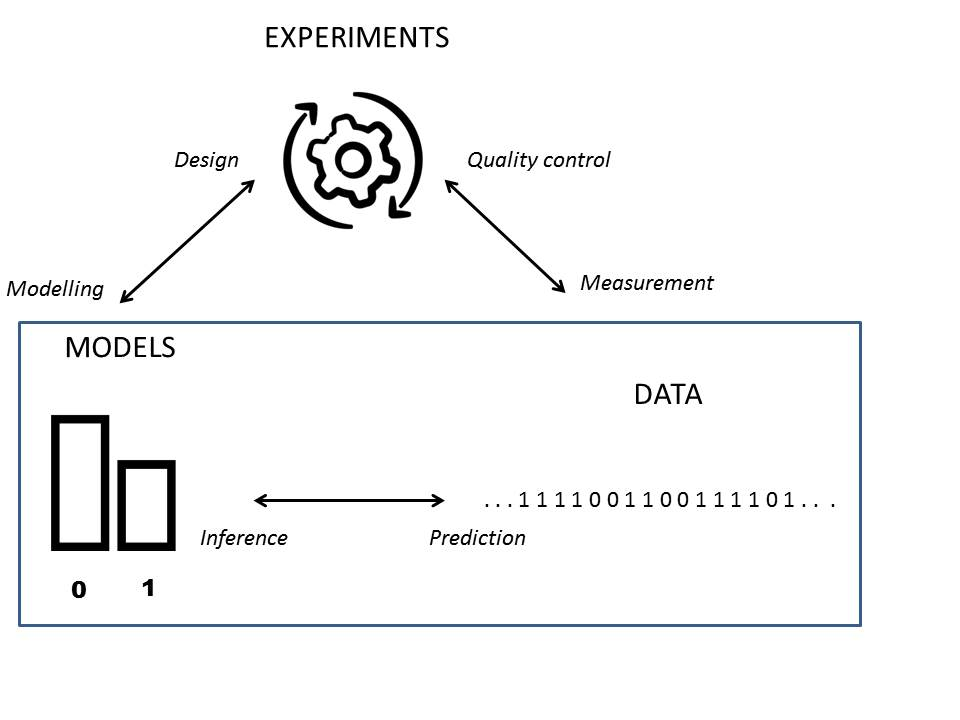
\includegraphics{./figures/stats.JPG}

\hypertarget{statistics}{%
\section{Statistics}\label{statistics}}

Statistics deals with the interaction between \emph{models} and \emph{data} (the bottom part of the figure).

The statistical questions are:

\begin{itemize}
\tightlist
\item
  What is the best model for my data (inference)?
\item
  What are the data that a certain model (prediction) would produce?
\end{itemize}

\hypertarget{data}{%
\section{Data}\label{data}}

The data is presented in the form of observations.

An \textbf{Observation} or \textbf{Realization} is the acquisition of a number or characteristic of an experiment.

For example, let's take the series of numbers produced by repeating an experiment (1: success, 0: failure).

\ldots{} 1 0 0 1 0 \textbf{1} 0 1 1 \ldots{}

The number in bold is \textbf{an observation} in a repeat of the experiment

An \textbf{outcome} is a \textbf{possible} observation that is the result of an experiment.

\textbf{1} is one result, \textbf{0} is the other result of the experiment.

Remember that the observation is \textbf{concrete} is the number you get one day in the laboratory. The \textbf{abstract} result is one of the characteristics of the type of experiment you are running.

\hypertarget{result-types}{%
\section{Result types}\label{result-types}}

In statistics we are mainly interested in two types of results.

\begin{itemize}
\item
  \textbf{Categorical}: If the result of an experiment is a quality. They can be nominal (binary: yes, no; multiple: colors) or ordinal when the qualities can be ranked (severity of a disease).
\item
  \textbf{Numeric}: If the result of an experiment is a number. The number can be discrete (number of emails received in an hour, number of leukocytes in the blood) or continuous (battery charge status, engine temperature).
\end{itemize}

\hypertarget{random-experiments}{%
\section{Random experiments}\label{random-experiments}}

It can be said that the subject of study of statistics is random experiments, the means by which we produce data.

\textbf{Definition:}

A \textbf{random experiment} is an experiment that gives different results when repeated in the same way.

Randomized experiments are of different types, depending on how they are conducted:

\begin{itemize}
\tightlist
\item
  on the same object (person): temperature, sugar levels.
  different objects but of the same size: the weight of an animal.
\item
  about events: the number of hurricanes per year.
\end{itemize}

\hypertarget{absolute-frequencies}{%
\section{Absolute frequencies}\label{absolute-frequencies}}

When we repeat a randomized experiment with \textbf{categorical} results, we record a list of results.

We summarize observations by counting how many times we saw a particular result.

\textbf{Absolute frecuency}:

\[ n_i \]

is the number of times we observe the result \(i\).

\newpage

\textbf{Example (leukocytes)}

Let's take a leukocyte from \textbf{a} donor and write down its type. Let's repeat the experiment \(N=119\) times.

\begin{verbatim}
(T cell, T cell, Neutrophil, ..., B cell)
\end{verbatim}

The second \textbf{T cell} in bold is the second observation. The last \textbf{B cell} is observation number 119.

We can list the \textbf{results} (categories) in a \textbf{frequency table}:

\begin{verbatim}
##      outcome ni
## 1     T Cell 34
## 2     B cell 50
## 3   basophil 20
## 4   Monocyte  5
## 5 Neutrophil 10
\end{verbatim}

From the table, we can say that, for example, \(n_1=34\) is the total number of T cells observed in the repeat experiment. We also note that the total number of repetitions \(N=\sum_i n_i = 119\).

\hypertarget{relative-frequencies}{%
\section{Relative frequencies}\label{relative-frequencies}}

We can also summarize observations by calculating the \textbf{proportion} of how many times we saw a particular result.

\[ f_i = n_i /N\] where \(N\) is the total number of observations

In our example, \(n_1=34\) T cells were recorded, so we asked about the proportion of T cells out of the total \(119\). We can add these proportions \(f_i\) in the frequency table.

\begin{verbatim}
##      outcome ni         fi
## 1     T Cell 34 0.28571429
## 2     B cell 50 0.42016807
## 3   basophil 20 0.16806723
## 4   Monocyte  5 0.04201681
## 5 Neutrophil 10 0.08403361
\end{verbatim}

Relative frequencies are \textbf{fundamental} in statistics. They give the proportion of one result in relation to the other results. Later we will understand them as the observations of probabilities.

For absolute and relative frequencies we have the properties

\begin{itemize}
\tightlist
\item
  \(\sum_{i=1..M} n_i = N\)
\item
  \(\sum_{i=1..M} f_i = 1\)
\end{itemize}

where \(M\) is the number of results.

\hypertarget{bar-chart}{%
\section{Bar chart}\label{bar-chart}}

When we have a lot of results and want to see which ones are most likely, we can use a bar chart that is a number of \(n_i\) Vs the results.

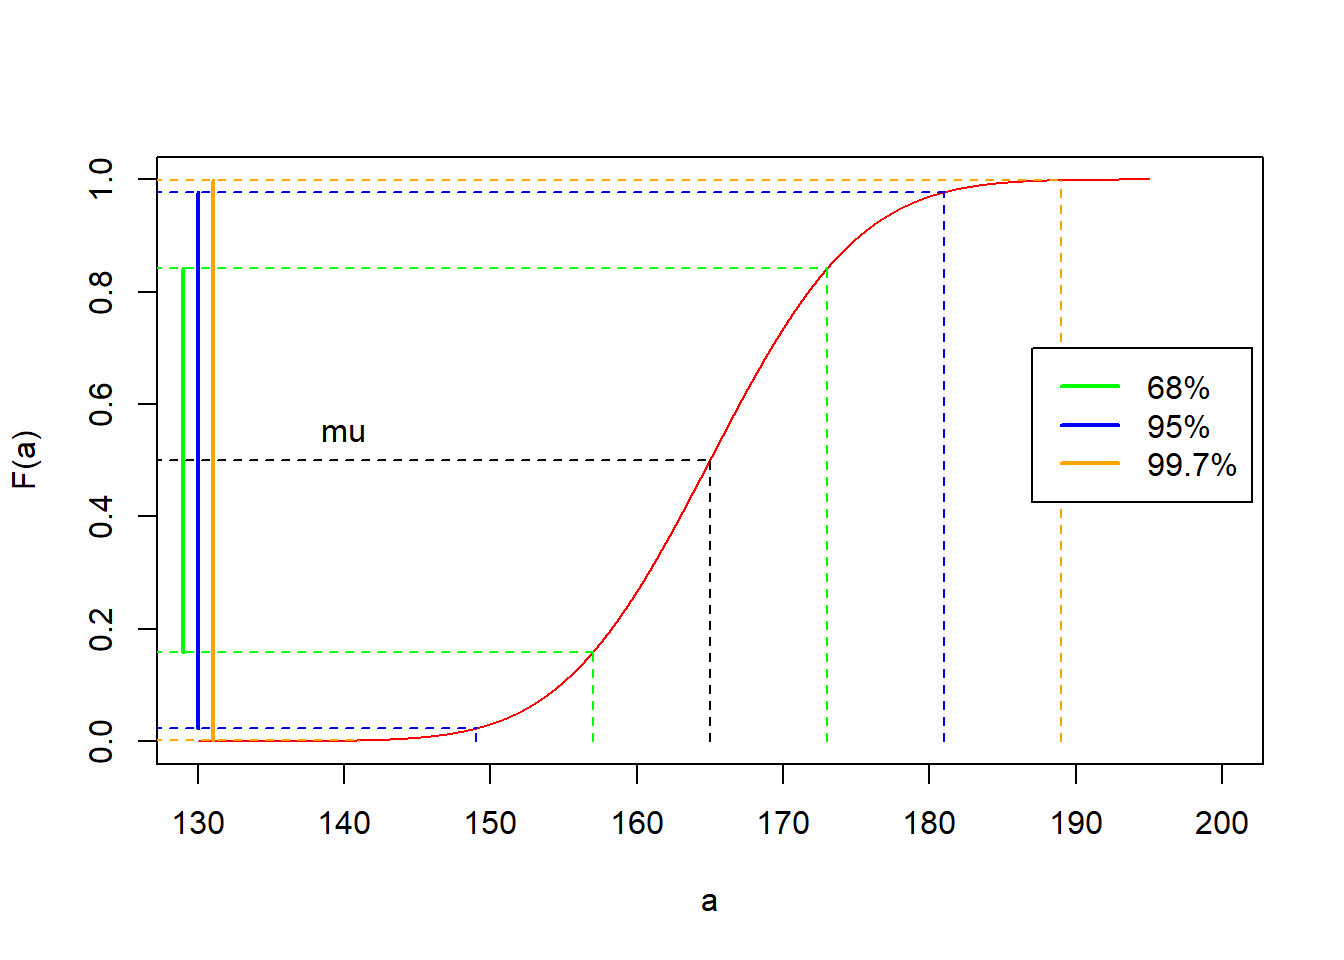
\includegraphics{_main_files/figure-latex/unnamed-chunk-3-1.pdf}

\hypertarget{pie-chart-pie}{%
\section{Pie chart (pie)}\label{pie-chart-pie}}

We can also visualize the relative frequencies with a pie chart.

The area of the circle represents 100\% of the observations (proportion = 1) and the sections the relative frequencies of each result.

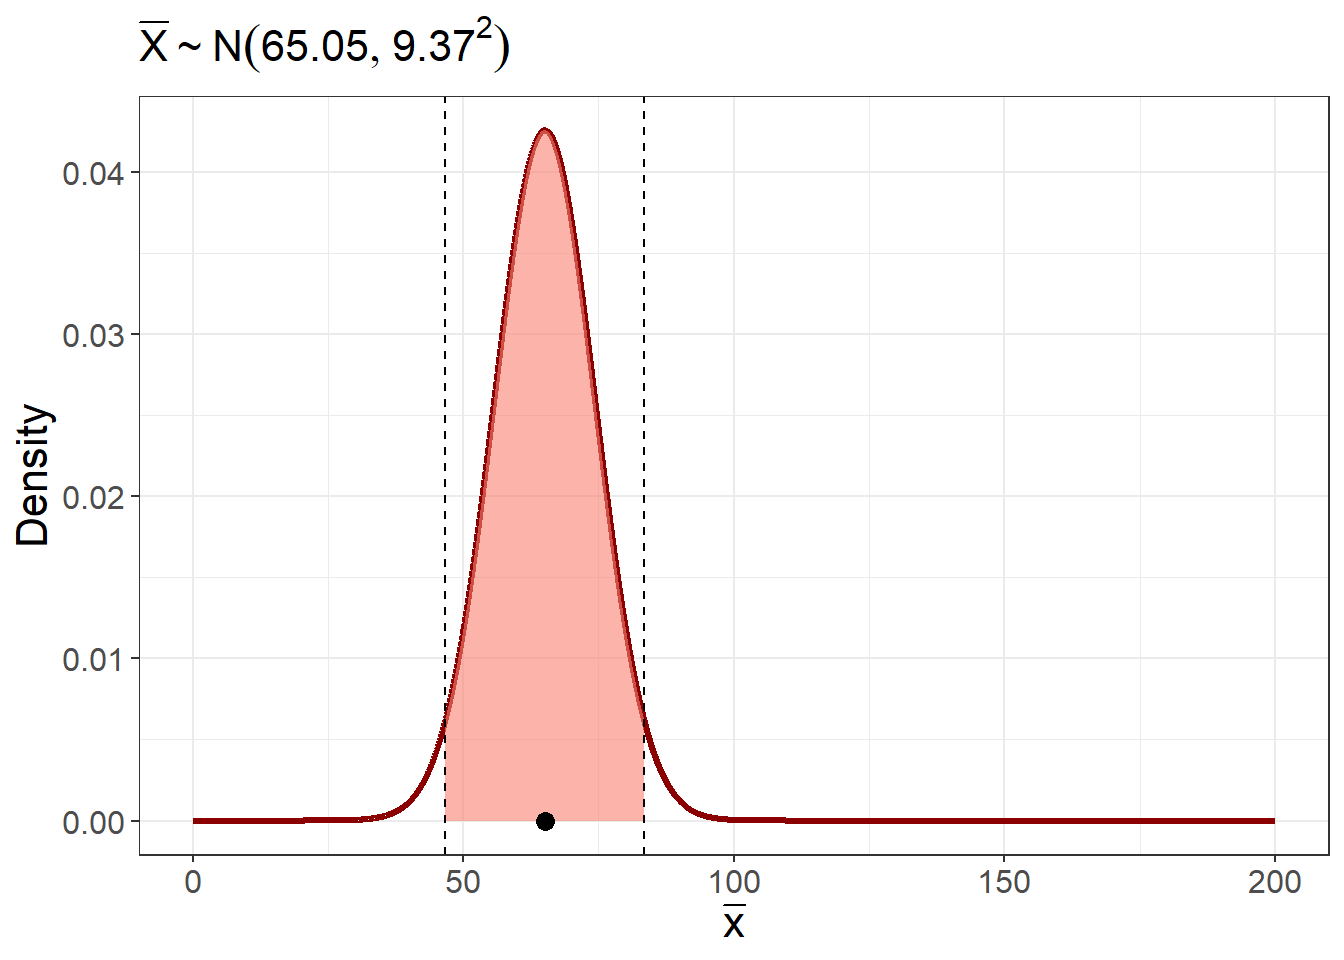
\includegraphics{_main_files/figure-latex/unnamed-chunk-4-1.pdf}

\hypertarget{ordinal-categorical-variables}{%
\section{Ordinal categorical variables}\label{ordinal-categorical-variables}}

The leukocyte type in the above examples is a \textbf{categorical} nominal variable. Each observation belongs to a category (quality). The categories do not always have a certain order .

Sometimes \textbf{categorical} variables can be \textbf{sorted} when they meet a natural ranking. This allows you to compute \textbf{cumulative frequencies}.

\newpage

\textbf{Example (Misophonia)}

This is a clinical study on 123 patients who were examined for their degree of misophonia. Misophnia is uncontrolled anxiety/anger produced by certain sounds .

Each patient was evaluated with a questionnaire (AMISO) and they were classified into 4 different groups according to severity.

The results of the study are

\begin{verbatim}
##   [1] 4 2 0 3 0 0 2 3 0 3 0 2 2 0 2 0 0 3 3 0 3 3 2 0 0 0 4 2 2 0 2 0 0 0 3 0 2
##  [38] 3 2 2 0 2 3 0 0 2 2 3 3 0 0 4 3 3 2 0 2 0 0 0 2 2 0 0 2 3 0 1 3 2 4 3 2 3
##  [75] 0 2 3 2 4 1 2 0 2 0 2 0 2 2 4 3 0 3 0 0 0 2 2 1 3 0 0 3 2 1 3 0 4 4 2 3 3
## [112] 3 0 3 2 1 2 3 3 4 2 3 2
\end{verbatim}

Each observation is the result of a randomized experiment: measurement of the level of misophonia in a patient. This data series can be summarized in terms of the results in the frequency table

\begin{verbatim}
##   outcome ni         fi
## 1       0 41 0.33333333
## 2       1  5 0.04065041
## 3       2 37 0.30081301
## 4       3 31 0.25203252
## 5       4  9 0.07317073
\end{verbatim}

\hypertarget{accumulated-absolute-and-relative-frequencies}{%
\section{Accumulated absolute and relative frequencies}\label{accumulated-absolute-and-relative-frequencies}}

Misophonia severity is \textbf{categorical} \textbf{ordinal} because its results can be ordered relative to its degree.

When the results can be ordered, it is useful to ask how many observations were obtained up to a given result. We call this number the \textbf{absolute cumulative frequency} up to the result \(i\):
\[N_i =\sum_{k= 1..i } n_k\]
It is also useful for calculating the \textbf{proportion} of observations up to a given result.

\[F_i =\sum_{k= 1..i } f_k\]

We can add these frequencies in the \textbf{frequency table}

\begin{verbatim}
##   outcome ni         fi  Ni        Fi
## 0       0 41 0.33333333  41 0.3333333
## 1       1  5 0.04065041  46 0.3739837
## 2       2 37 0.30081301  83 0.6747967
## 3       3 31 0.25203252 114 0.9268293
## 4       4  9 0.07317073 123 1.0000000
\end{verbatim}

Therefore, \textbf{67\%} of patients had misophonia up to severity \textbf{2} and \textbf{37\%} of patients had severity less than or equal to \textbf{1}.

\hypertarget{cumulative-frequency-graph}{%
\section{Cumulative frequency graph}\label{cumulative-frequency-graph}}

\(F_i\) is an important quantity because it allows us to define the accumulation of probabilities down to intermediate levels.

The probability of an intermediate level \(x\) (\(i\leq x< i+1\)) is just the accumulation up to the lower level \(F_x = F_i\).

\(F_x\) is therefore a function on a \textbf{continuous} range of values. We can draw it with respect to the results.

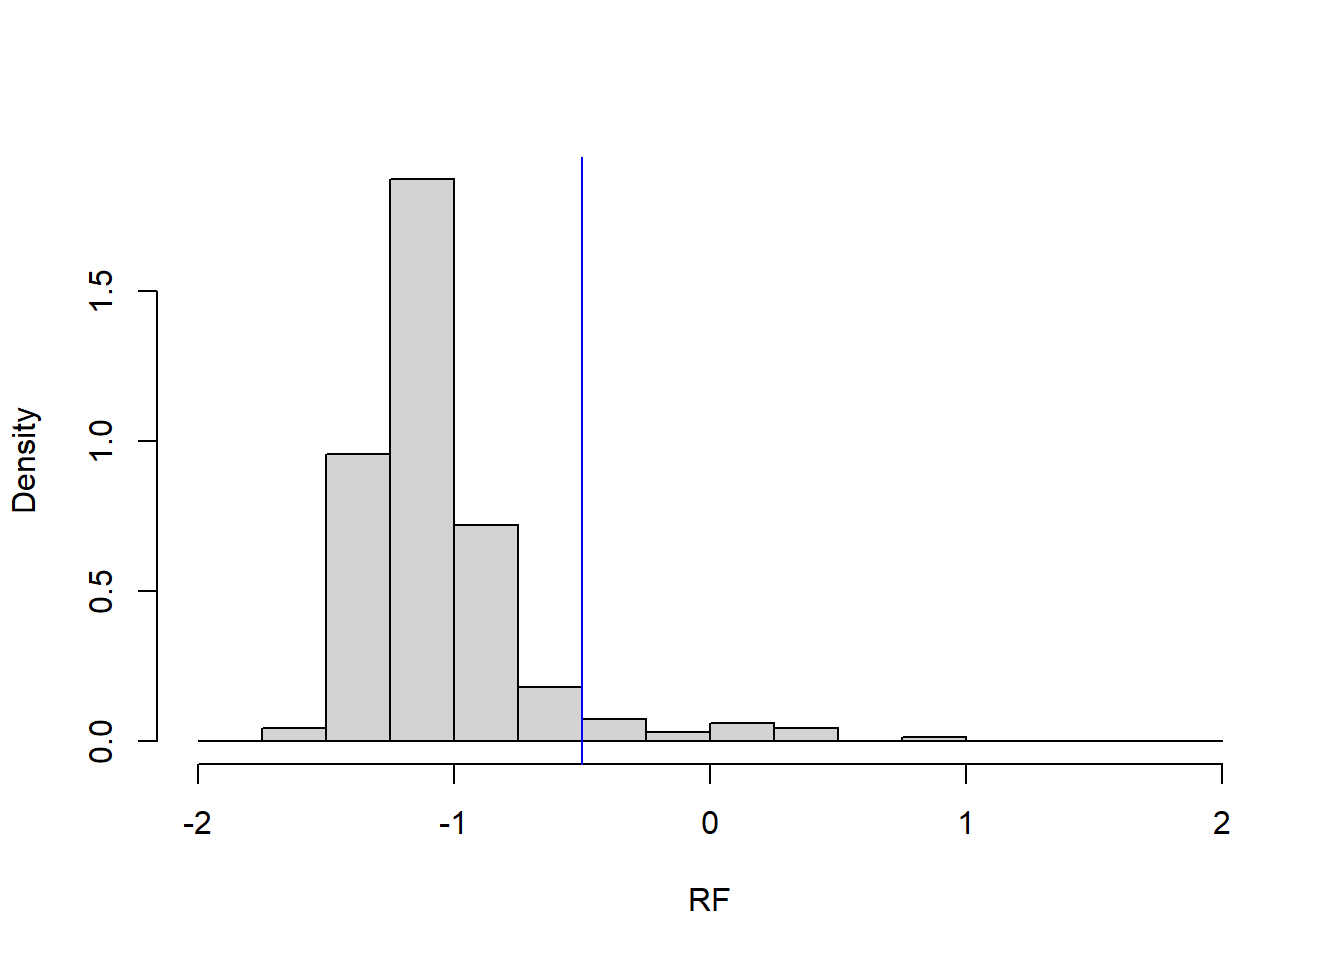
\includegraphics{_main_files/figure-latex/unnamed-chunk-8-1.pdf}

Therefore, we can say that \textbf{67\%} of the patients had misophonia up to severity \(2.3\), although \(2.3\) is not an observed outcome.

\hypertarget{numeric-variables}{%
\section{Numeric variables}\label{numeric-variables}}

The result of a random experiment can produce a number. If the number is \textbf{discrete}, we can generate a frequency table, with absolute, relative, and cumulative frequencies, and illustrate them with bar, pie, and cumulative charts.

When the number is \textbf{continuous} the frequencies are not useful, we are most likely to observe or not observe a particular continuous number.

\textbf{Example (misophonia)}

The researchers wondered if the convexity of the jaw would affect the severity of misophonia. The scientific hypothesis is that the angle of convexity of the jaw can influence hearing and its sensitivity. These are the mandibular convexity results (degrees) for each patient:

\begin{verbatim}
##   [1]  7.97 18.23 12.27  7.81  9.81 13.50 19.30  7.70 12.30  7.90 12.60 19.00
##  [13]  7.27 14.00  5.40  8.00 11.20  7.75  7.94 16.69  7.62  7.02  7.00 19.20
##  [25]  7.96 14.70  7.24  7.80  7.90  4.70  4.40 14.00 14.40 16.00  1.40  9.76
##  [37]  7.90  7.90  7.40  6.30  7.76  7.30  7.00 11.23 16.00  7.90  7.29  6.91
##  [49]  7.10 13.40 11.60 -1.00  6.00  7.82  4.80 11.00  9.00 11.50 16.00 15.00
##  [61]  1.40 16.80  7.70 16.14  7.12 -1.00 17.00  9.26 18.70  3.40 21.30  7.50
##  [73]  6.03  7.50 19.00 19.01  8.10  7.80  6.10 15.26  7.95 18.00  4.60 15.00
##  [85]  7.50  8.00 16.80  8.54  7.00 18.30  7.80 16.00 14.00 12.30 11.40  8.50
##  [97]  7.00  7.96 17.60 10.00  3.50  6.70 17.00 20.26  6.64  1.80  7.02  2.46
## [109] 19.00 17.86  6.10  6.64 12.00  6.60  8.70 14.05  7.20 19.70  7.70  6.02
## [121]  2.50 19.00  6.80
\end{verbatim}

\hypertarget{transforming-continuous-data}{%
\section{Transforming continuous data}\label{transforming-continuous-data}}

Since continuous outcomes cannot be counted (informatively), we transform them into ordered categorical variables.

\begin{enumerate}
\def\labelenumi{\arabic{enumi})}
\tightlist
\item
  First we cover the range of observations in regular intervals of the same size (bins)
\end{enumerate}

\begin{verbatim}
## [1] "[-1.02,3.46]" "(3.46,7.92]"  "(7.92,12.4]"  "(12.4,16.8]"  "(16.8,21.3]"
\end{verbatim}

\begin{enumerate}
\def\labelenumi{\arabic{enumi})}
\setcounter{enumi}{1}
\tightlist
\item
  Then we map each observation to its interval: creating a categorical variable \textbf{ordered}; in this case with 5 possible outcomes
\end{enumerate}

\begin{verbatim}
##   [1] "(7.92,12.4]"  "(16.8,21.3]"  "(7.92,12.4]"  "(3.46,7.92]"  "(7.92,12.4]" 
##   [6] "(12.4,16.8]"  "(16.8,21.3]"  "(3.46,7.92]"  "(7.92,12.4]"  "(3.46,7.92]" 
##  [11] "(12.4,16.8]"  "(16.8,21.3]"  "(3.46,7.92]"  "(12.4,16.8]"  "(3.46,7.92]" 
##  [16] "(7.92,12.4]"  "(7.92,12.4]"  "(3.46,7.92]"  "(7.92,12.4]"  "(12.4,16.8]" 
##  [21] "(3.46,7.92]"  "(3.46,7.92]"  "(3.46,7.92]"  "(16.8,21.3]"  "(7.92,12.4]" 
##  [26] "(12.4,16.8]"  "(3.46,7.92]"  "(3.46,7.92]"  "(3.46,7.92]"  "(3.46,7.92]" 
##  [31] "(3.46,7.92]"  "(12.4,16.8]"  "(12.4,16.8]"  "(12.4,16.8]"  "[-1.02,3.46]"
##  [36] "(7.92,12.4]"  "(3.46,7.92]"  "(3.46,7.92]"  "(3.46,7.92]"  "(3.46,7.92]" 
##  [41] "(3.46,7.92]"  "(3.46,7.92]"  "(3.46,7.92]"  "(7.92,12.4]"  "(12.4,16.8]" 
##  [46] "(3.46,7.92]"  "(3.46,7.92]"  "(3.46,7.92]"  "(3.46,7.92]"  "(12.4,16.8]" 
##  [51] "(7.92,12.4]"  "[-1.02,3.46]" "(3.46,7.92]"  "(3.46,7.92]"  "(3.46,7.92]" 
##  [56] "(7.92,12.4]"  "(7.92,12.4]"  "(7.92,12.4]"  "(12.4,16.8]"  "(12.4,16.8]" 
##  [61] "[-1.02,3.46]" "(12.4,16.8]"  "(3.46,7.92]"  "(12.4,16.8]"  "(3.46,7.92]" 
##  [66] "[-1.02,3.46]" "(16.8,21.3]"  "(7.92,12.4]"  "(16.8,21.3]"  "[-1.02,3.46]"
##  [71] "(16.8,21.3]"  "(3.46,7.92]"  "(3.46,7.92]"  "(3.46,7.92]"  "(16.8,21.3]" 
##  [76] "(16.8,21.3]"  "(7.92,12.4]"  "(3.46,7.92]"  "(3.46,7.92]"  "(12.4,16.8]" 
##  [81] "(7.92,12.4]"  "(16.8,21.3]"  "(3.46,7.92]"  "(12.4,16.8]"  "(3.46,7.92]" 
##  [86] "(7.92,12.4]"  "(12.4,16.8]"  "(7.92,12.4]"  "(3.46,7.92]"  "(16.8,21.3]" 
##  [91] "(3.46,7.92]"  "(12.4,16.8]"  "(12.4,16.8]"  "(7.92,12.4]"  "(7.92,12.4]" 
##  [96] "(7.92,12.4]"  "(3.46,7.92]"  "(7.92,12.4]"  "(16.8,21.3]"  "(7.92,12.4]" 
## [101] "(3.46,7.92]"  "(3.46,7.92]"  "(16.8,21.3]"  "(16.8,21.3]"  "(3.46,7.92]" 
## [106] "[-1.02,3.46]" "(3.46,7.92]"  "[-1.02,3.46]" "(16.8,21.3]"  "(16.8,21.3]" 
## [111] "(3.46,7.92]"  "(3.46,7.92]"  "(7.92,12.4]"  "(3.46,7.92]"  "(7.92,12.4]" 
## [116] "(12.4,16.8]"  "(3.46,7.92]"  "(16.8,21.3]"  "(3.46,7.92]"  "(3.46,7.92]" 
## [121] "[-1.02,3.46]" "(16.8,21.3]"  "(3.46,7.92]"
\end{verbatim}

Therefore, instead of saying that the first patient had an angle of convexity of \(7.97\), we say that his angle was between the interval (or \textbf{bin}) \((7.92,12.4]\).

No other patients had an angle of \(7.97\), but many had angles between \((7.92,12.4]\).

\hypertarget{frequency-table-for-a-continuous-variable}{%
\section{Frequency table for a continuous variable}\label{frequency-table-for-a-continuous-variable}}

For a given regular partition of the interval of results into intervals, we can produce a frequency table as before

\begin{verbatim}
##        outcome ni         fi  Ni         Fi
## 1 [-1.02,3.46]  8 0.06504065   8 0.06504065
## 2  (3.46,7.92] 51 0.41463415  59 0.47967480
## 3  (7.92,12.4] 26 0.21138211  85 0.69105691
## 4  (12.4,16.8] 20 0.16260163 105 0.85365854
## 5  (16.8,21.3] 18 0.14634146 123 1.00000000
\end{verbatim}

\hypertarget{histogram}{%
\section{Histogram}\label{histogram}}

The histogram is the graph of \(n_i\) or \(f_i\) Vs the results in intervals (bins). The histogram depends on the size of the bins .

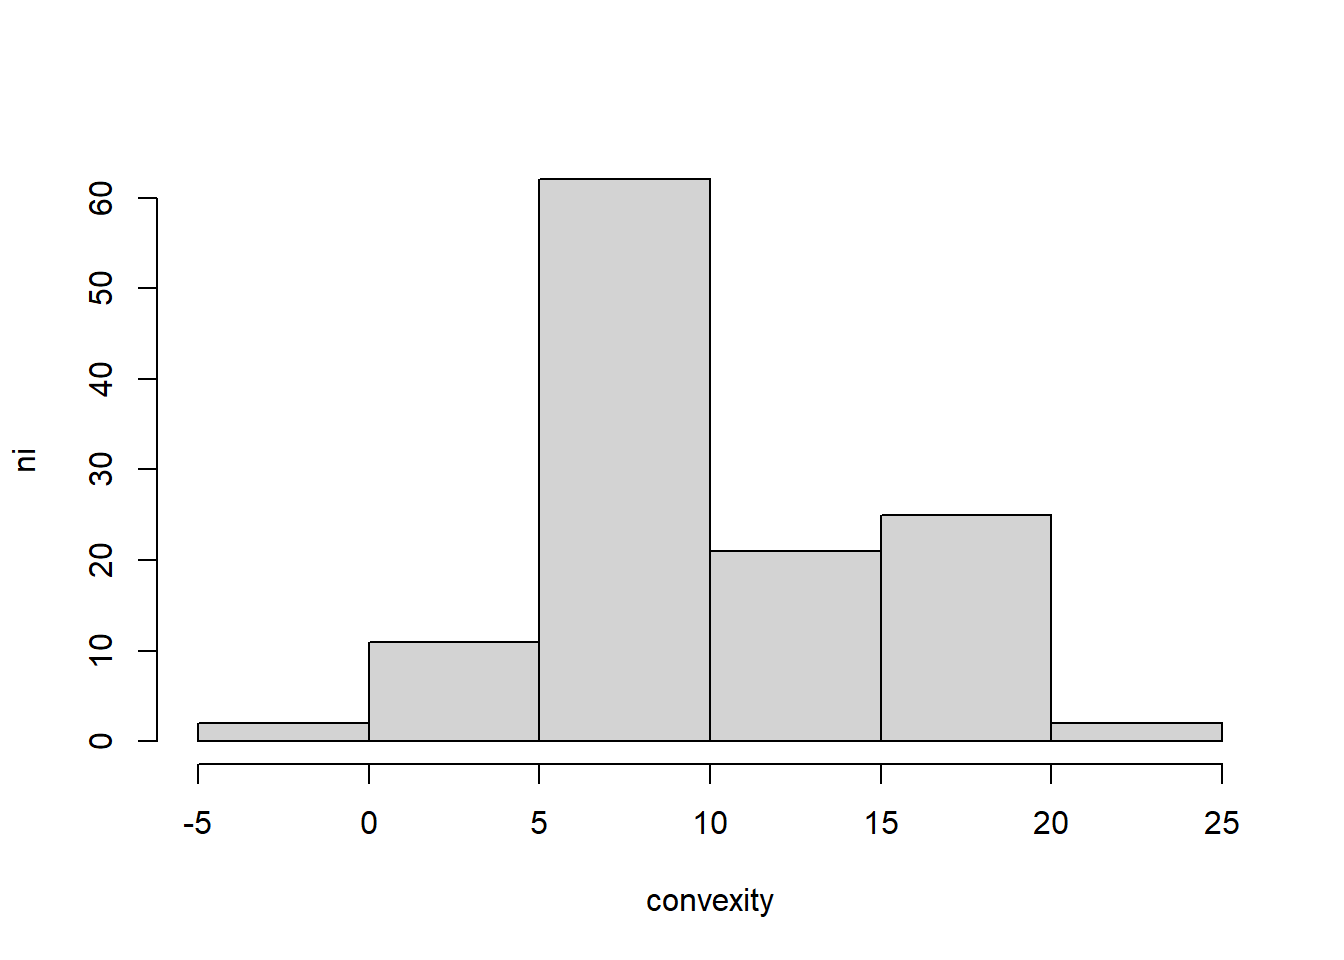
\includegraphics{_main_files/figure-latex/unnamed-chunk-13-1.pdf}

\newpage

This is a histogram with 20 bins .

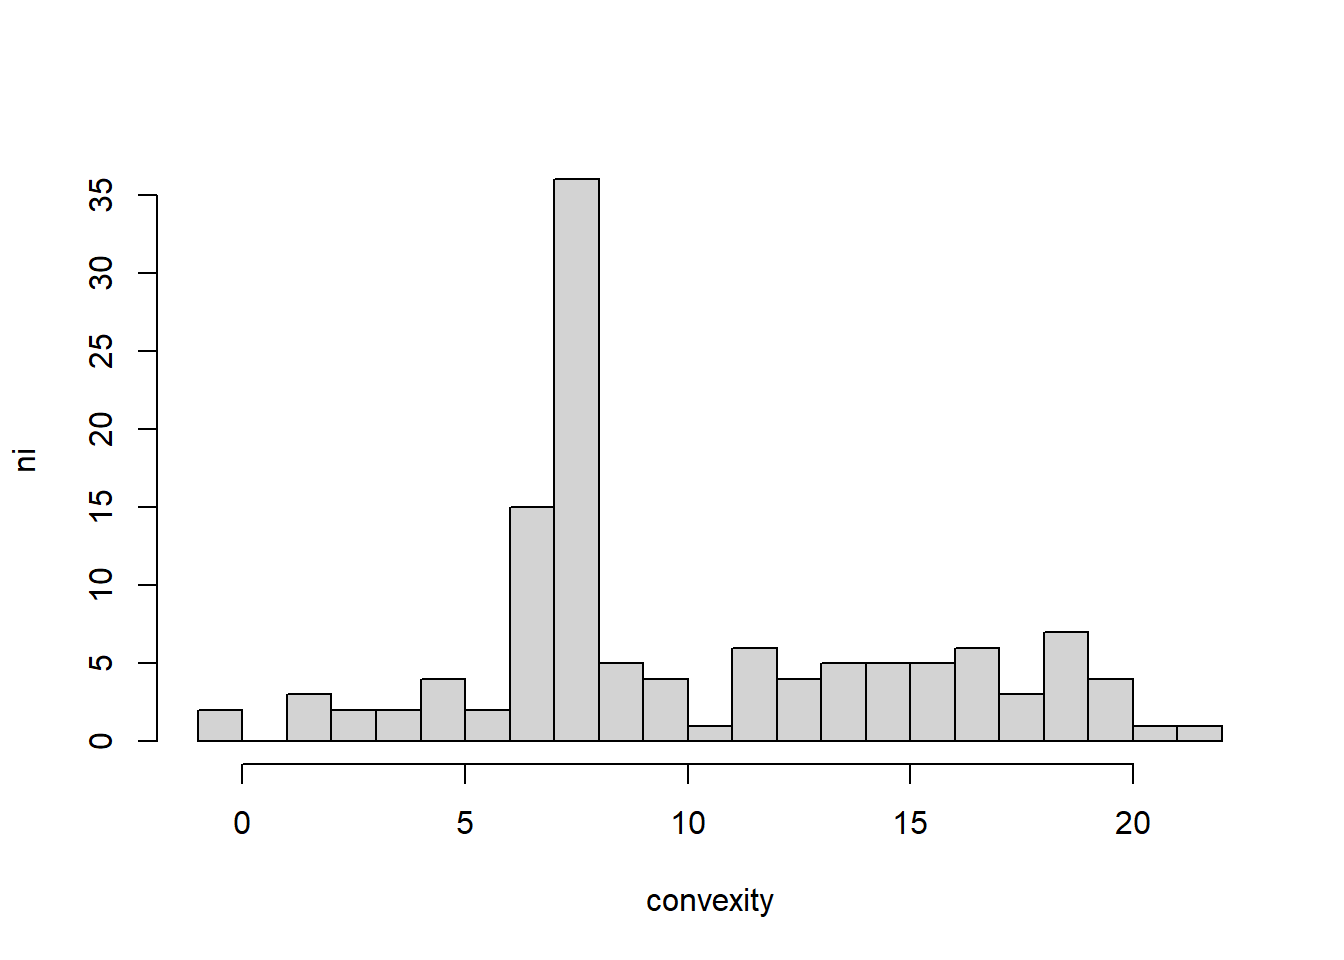
\includegraphics{_main_files/figure-latex/unnamed-chunk-14-1.pdf}

We see that most people have angles within \((7, 8]\)

\hypertarget{cumulative-frequency-graph-1}{%
\section{Cumulative frequency graph}\label{cumulative-frequency-graph-1}}

We can also plot \(F_x\) against the results. Since \(F_x\) is of continuous range, we can order the observations (\(x_1 <... x_j < x_{j+1} < x_n\)) and therefore

\[F_x = \frac{k}{ n}\]

for \(x_{k} \leq x < x_{k+ 1}\) .

\(F_x\) is known as the \textbf{distribution} of the data. \(F_x\) does not depend on the size of the bin. However, its \textbf{resolution} depends on the amount of data.

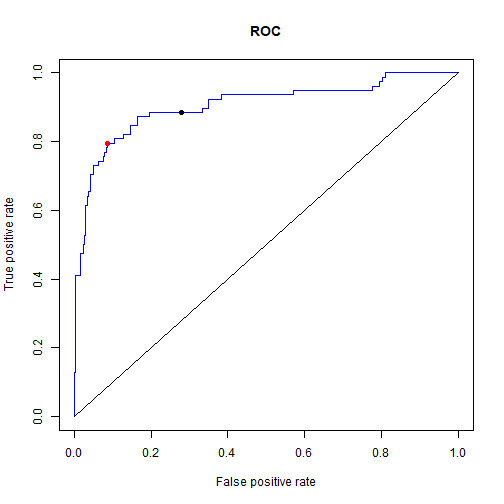
\includegraphics{_main_files/figure-latex/unnamed-chunk-15-1.pdf}

\hypertarget{summary-statistics}{%
\section{Summary Statistics}\label{summary-statistics}}

Summary statistics are numbers calculated from the data that tell us important characteristics of the numerical variables (discrete or continuous).

For example, we have statistics that describe extreme values:

\begin{itemize}
\tightlist
\item
  \textbf{minimum}: the minimum result observed
\item
  \textbf{maximum}: the maximum result observed
\end{itemize}

\hypertarget{average-sample-mean}{%
\section{Average (sample mean)}\label{average-sample-mean}}

An important statistic that describes the central value of the results (where to expect most observations) is the \textbf{average}

\[\bar{x}=\frac{1}{N} \sum_{j= 1..N } x_j \]

where \(x_j\) is the \textbf{observation} \(j\) out of a total of \(N\).

\textbf{Example (Misophonia)}

The average convexity can be calculated directly from the \textbf{observations} in the usual way

\(\bar{x}= \frac{1}{ N}\sum_j x_j\)

\(= \frac{1}{ N}( 7.97 + 18.23 + 12.27... + 6.80) = 10.19894\)

For \textbf{categorically ordered} variables, we can \textbf{also} use the relative frequencies to calculate the average

\(\bar{x}=\frac{1}{ N}\sum_{i=1...N} x_j =\frac{1}{N}\sum_{i=1...M} x_i n_ {i}=\)
\[\sum_{i=1...M} x_i f_{i}\]

where we went from adding \(N\) \textbf{observations} to adding \(M\) \textbf{results}.

The form \(\bar{x}= \sum_{i = 1...M} x_i f_i\) shows that the average is the \textbf{center of gravity} of the results. As if each result had a mass density given by \(f_i\).

\textbf{Example (Misophonia)}

The average \textbf{severity} of misophonia in the study can be calculated from the relative frequencies of the \textbf{outcomes}

\begin{verbatim}
##   outcome ni         fi
## 1       0 41 0.33333333
## 2       1  5 0.04065041
## 3       2 37 0.30081301
## 4       3 31 0.25203252
## 5       4  9 0.07317073
\end{verbatim}

\(\bar{x}=0*f_ {0}+ 1*f_{1}+2*f_{2}+3*f_{3}+4*f_{4}=1.691057\)

The average is also the center of gravity for continuous variables. That is the point where the relative frequencies balance.

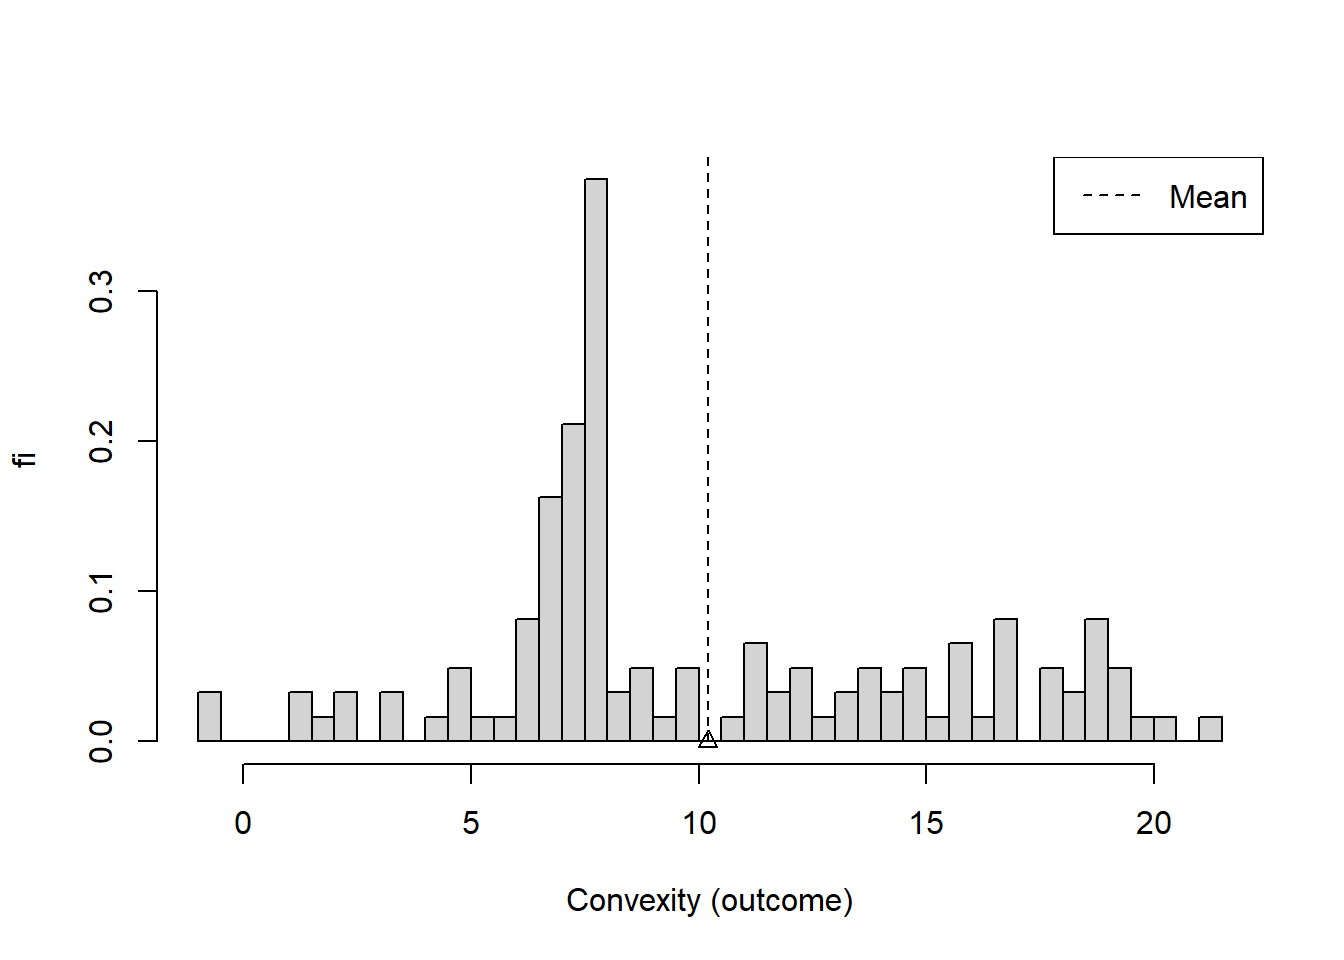
\includegraphics{_main_files/figure-latex/unnamed-chunk-17-1.pdf}

\hypertarget{median}{%
\section{Median}\label{median}}

Another measure of centrality is the median. The median \(x_m\), or \(q_{0.5}\), is the value below which we find half of the observations. When we order the observations \(x_1 <... x_j < x_{j+1} < x_N\), we count them until we find half of them. Therefore, \(x_m\) is the observation such that \(m\) satisfies

\[\sum_{i\leq m} 1 = \frac{N}{2}\]
\textbf{Example (Misophonia)}

If we order the angles of convexity, we see that \(62\) observations (individuals) (\(N/2 \sim 123/2\)) are below \(7.96\). The \textbf{median convexity} is therefore \(q_{0.5}= x_{62}=7.96\)

\begin{verbatim}
##  [1] -1.00 -1.00  1.40  1.40  1.80  2.46  2.50  3.40  3.50  4.40  4.60  4.70
## [13]  4.80  5.40  6.00  6.02  6.03  6.10  6.10  6.30  6.60  6.64  6.64  6.70
## [25]  6.80  6.91  7.00  7.00  7.00  7.00  7.02  7.02  7.10  7.12  7.20  7.24
## [37]  7.27  7.29  7.30  7.40  7.50  7.50  7.50  7.62  7.70  7.70  7.70  7.75
## [49]  7.76  7.80  7.80  7.80  7.81  7.82  7.90  7.90  7.90  7.90  7.90  7.94
## [61]  7.95  7.96
\end{verbatim}

\begin{verbatim}
##  [1]  7.96  7.97  8.00  8.00  8.10  8.50  8.54  8.70  9.00  9.26  9.76  9.81
## [13] 10.00 11.00 11.20 11.23 11.40 11.50 11.60 12.00 12.27 12.30 12.30 12.60
## [25] 13.40 13.50 14.00 14.00 14.00 14.05 14.40 14.70 15.00 15.00 15.26 16.00
## [37] 16.00 16.00 16.00 16.14 16.69 16.80 16.80 17.00 17.00 17.60 17.86 18.00
## [49] 18.23 18.30 18.70 19.00 19.00 19.00 19.00 19.01 19.20 19.30 19.70 20.26
## [61] 21.30
\end{verbatim}

We cut the data at

\begin{verbatim}
## [1] 7.96
\end{verbatim}

to split them in half.

\newpage

In terms of frequencies, \(q_{0.5}\) makes the cumulative frequency \(F_x\) equal to \(0.5\)

\[\sum_{i = 0, ... m} f_i =F_{q_{0.5}}=0.5\]
that is

\[q_{ 0.5}= F^{-1}(0.5)\]

This last equation means that, in the distribution graph, the median \(q_{ 0.5}\) is the value of \(x\) at which we have climbed half of the total height of \(F\).

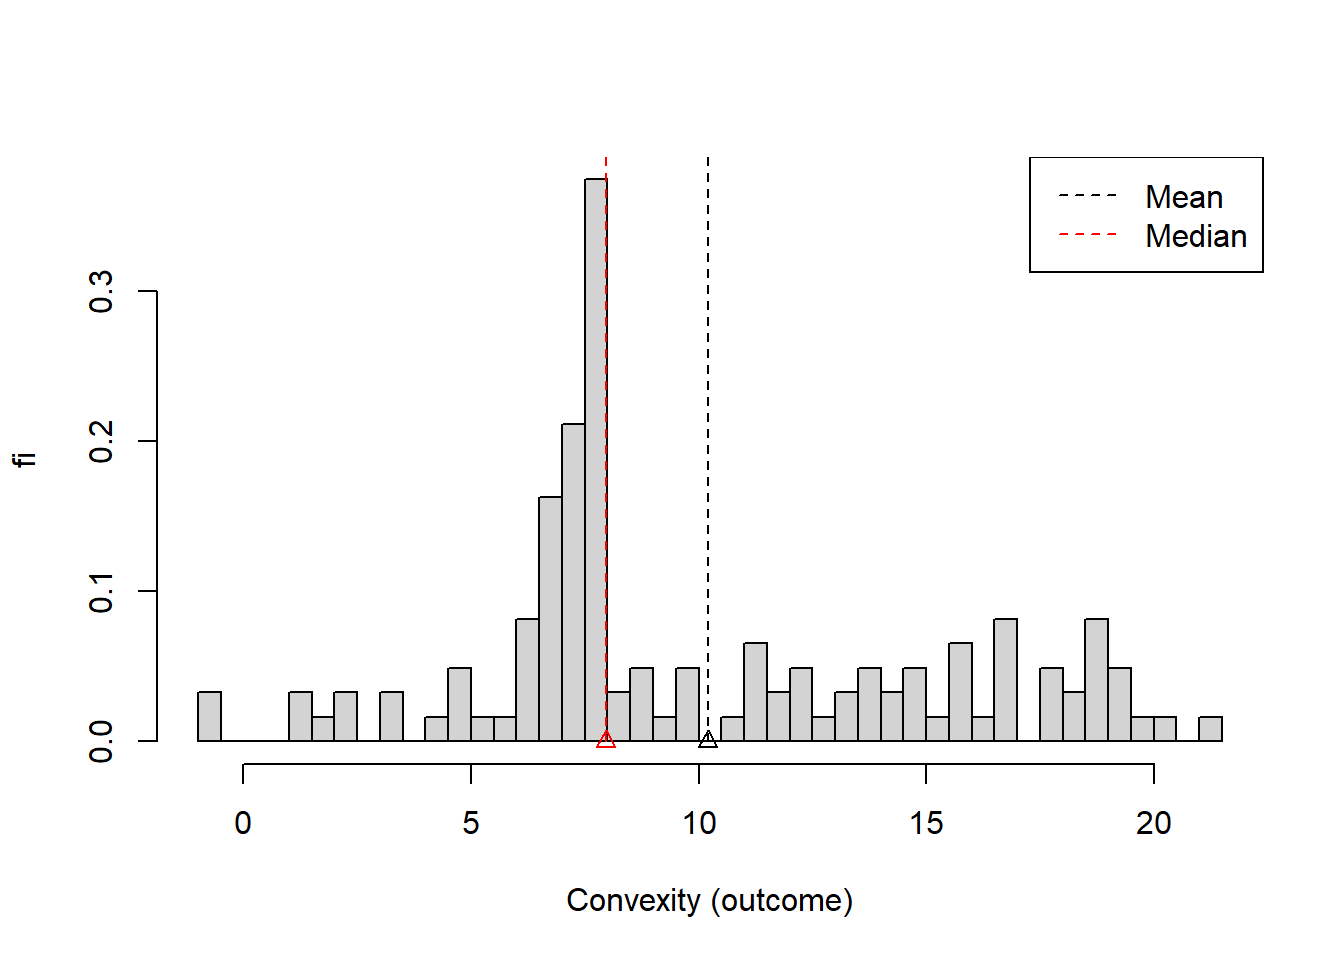
\includegraphics{_main_files/figure-latex/unnamed-chunk-21-1.pdf}

The mean and median are not always the same.

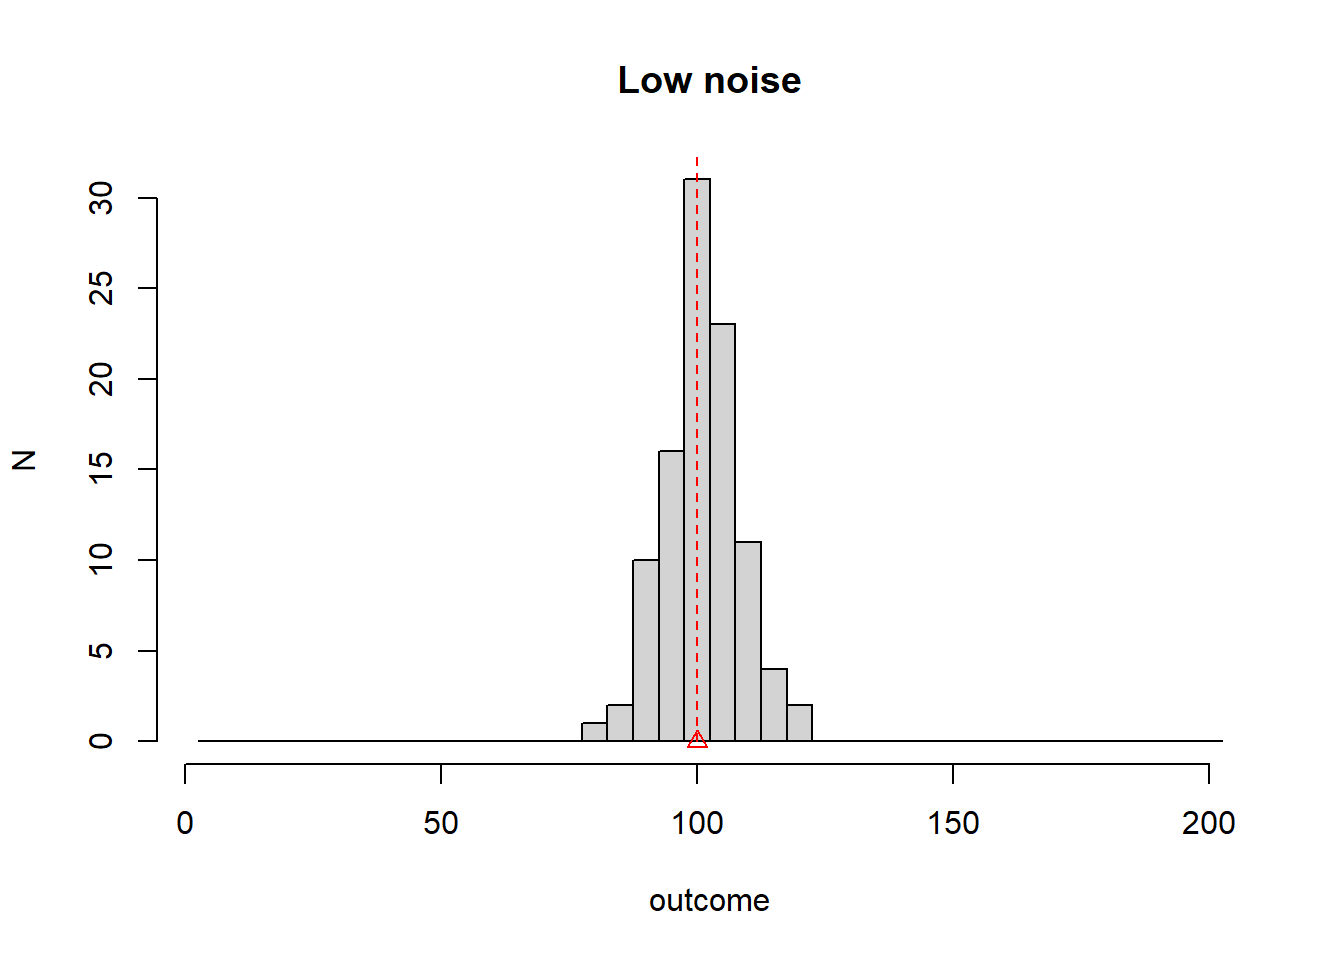
\includegraphics{_main_files/figure-latex/unnamed-chunk-22-1.pdf}

\hypertarget{dispersion}{%
\section{Dispersion}\label{dispersion}}

Other important summary statistics for observations are the \textbf{spread} statistics.

Many experiments may share their mean, but differ in how \textbf{sparse} the values are.

The dispersion of the observations is a measure of the \textbf{noise}.

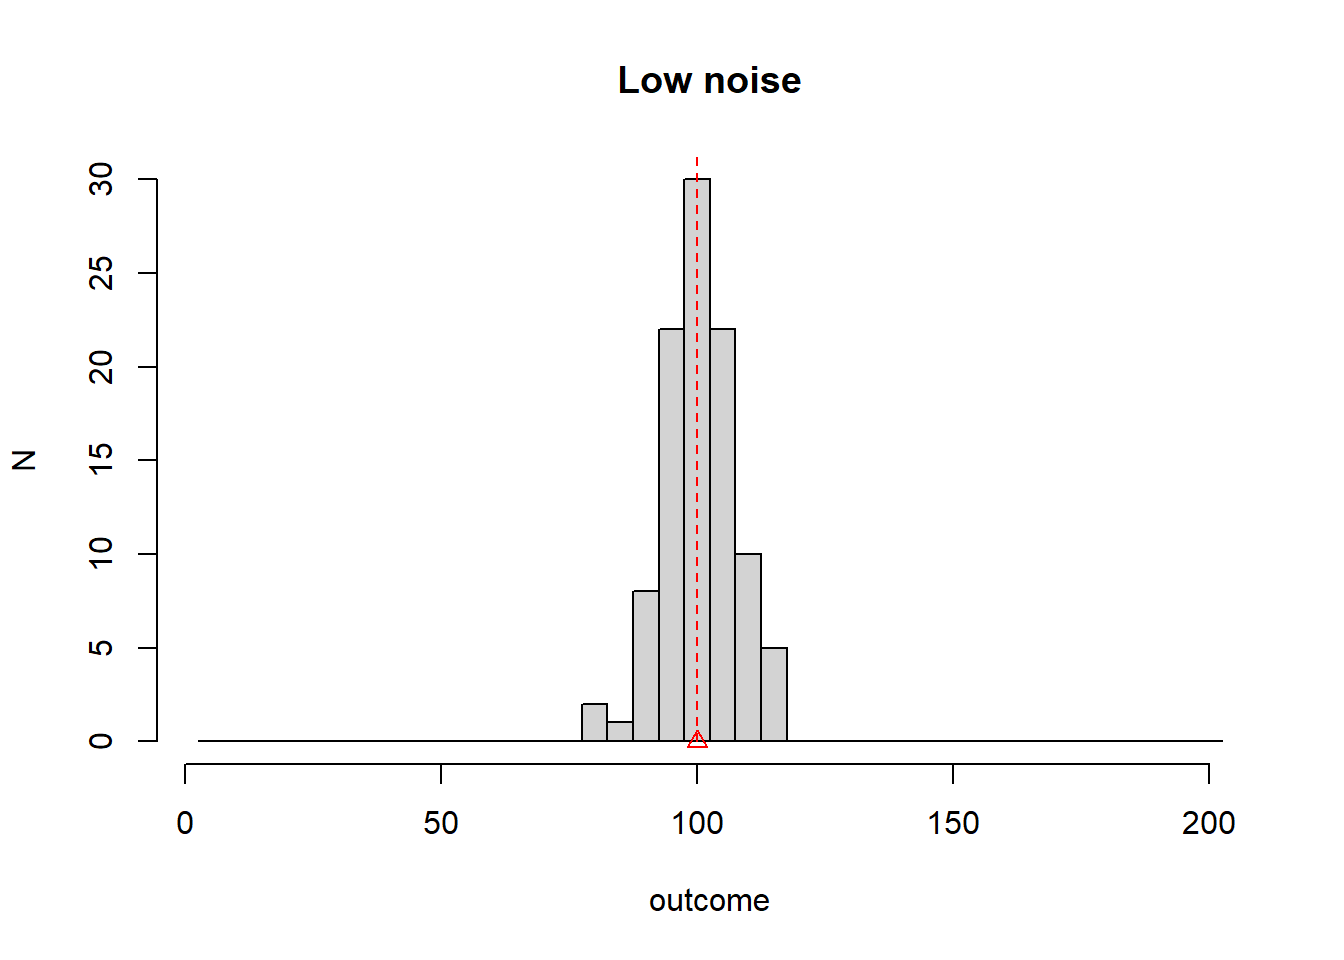
\includegraphics{_main_files/figure-latex/unnamed-chunk-23-1.pdf} 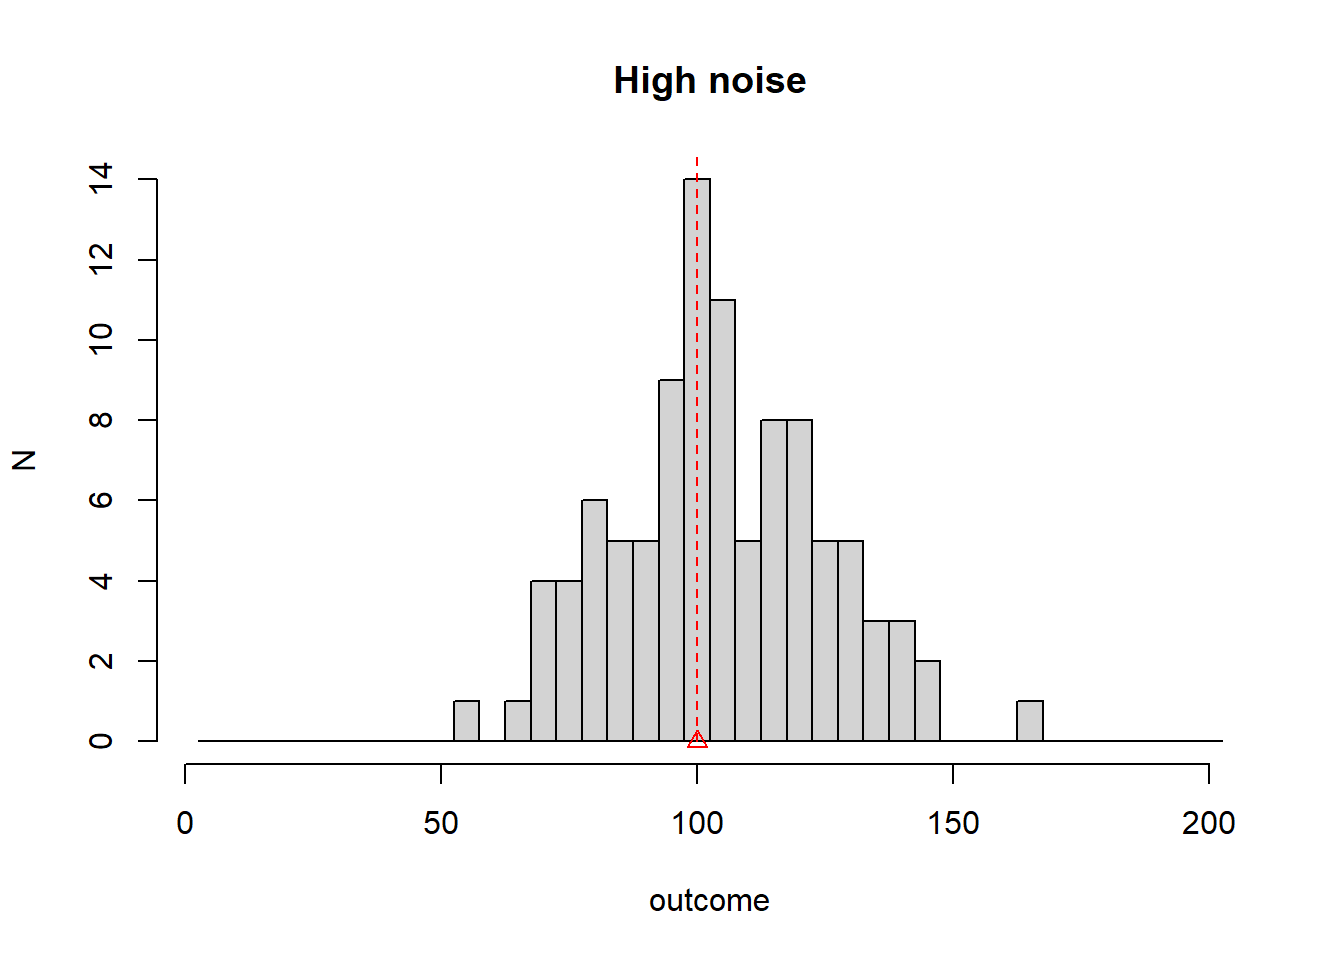
\includegraphics{_main_files/figure-latex/unnamed-chunk-23-2.pdf}

\hypertarget{sample-variance}{%
\section{Sample variance}\label{sample-variance}}

The dispersion about the mean is measured by the sample variance

\[s^2=\frac{ 1}{ N-1} \sum_{j=1..N} ( x_j -\bar{x})^2\]

This number measures the average squared distance of the \textbf{observations} from the average. The reason for \(N-1\) will be explained when we talk about inference, when we study the spread of \(\bar{x}\), as well as the spread of the observations.

In terms of the frequencies of the variables that are \textbf{categorical and ordered}, we can \textbf{also} calculate the sample variance as

\[s^2=\frac{N}{N-1} \sum_{i=1... M} (x_i -\bar{x})^2 f_i\]

\(s^2\) can be considered as the \textbf{moment of inertia} of the observations.

The square root of the sample variance, \(s\), is called \textbf{standard deviation} of the sample.

\textbf{Example (Misophonia)}

The standard deviation of the angle of convexity is

\(s= [\frac{ 1}{123-1}((7.97-10.19894)^2+ (18.23-10.19894)^2\)
\[+ (12.27-10.19894 )^ 2 + ...)]^{1/2} = 5.086707\]

The jaw convexity deviates from its mean by \(5.086707\).

\hypertarget{interquartile-range-iqr}{%
\section{Interquartile range (IQR)}\label{interquartile-range-iqr}}

The spread of the data can also be measured with respect to the median using the \textbf{interquartile range}:

\begin{enumerate}
\def\labelenumi{\arabic{enumi})}
\tightlist
\item
  We define the \textbf{first} quartile as the value \(x_m\) that makes the cumulative frequency \(F_{q_{0.25}}\) equal to \(0.25\) (or the value of \(x\) where we have accumulated a quarter of the observations, or the value that splits the first quarter of the observations)
\end{enumerate}

\[q_{0.25}=F^{-1}(0.25)\]

\begin{enumerate}
\def\labelenumi{\arabic{enumi})}
\setcounter{enumi}{1}
\tightlist
\item
  We define the \textbf{third} quartile as the value \(x_m\) that makes the cumulative frequency \(F_{q_{0.75}}\) equal to \(0.75\) (or the value of \(x\) where we have accumulated three quarters of observations)
\end{enumerate}

\[q_{0.75}=F^{-1}(0.75)\]

\begin{enumerate}
\def\labelenumi{\arabic{enumi})}
\setcounter{enumi}{2}
\tightlist
\item
  The \textbf{interquartile range} (IQR) is \[IQR=q_{0.75} - q_{0.25}\]
\end{enumerate}

This is the distance between the third and first quartiles and captures the central \(50\%\) of the observations

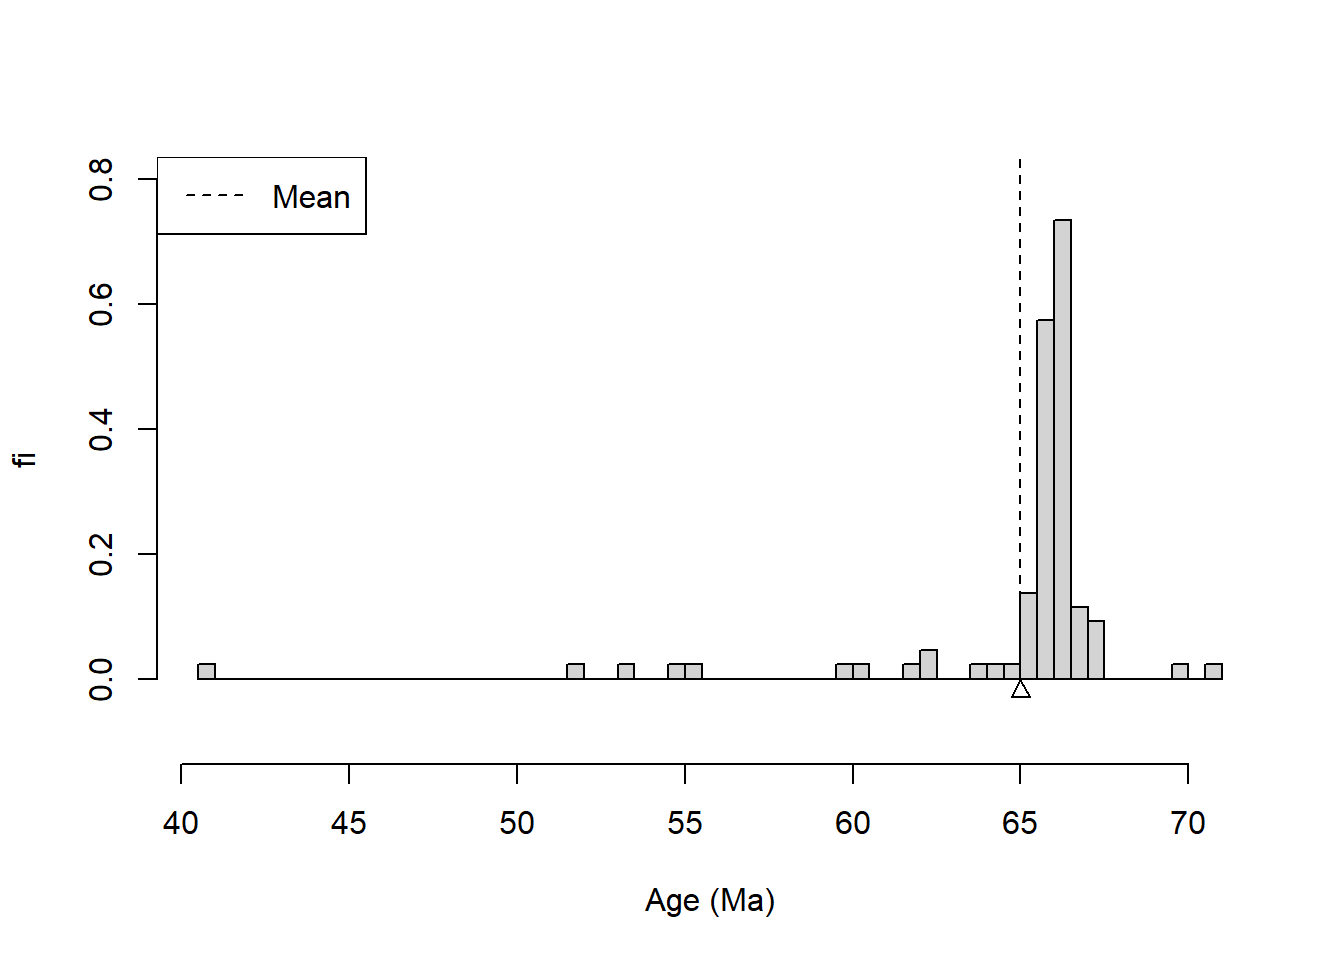
\includegraphics{_main_files/figure-latex/unnamed-chunk-24-1.pdf}

\hypertarget{boxplot}{%
\section{Boxplot}\label{boxplot}}

The interquartile range, median, and \(5\%\) and \(95\%\) of the data can be displayed in a \textbf{box plot}.

In the boxplot, the values of the results are on the y-axis. The IQR is the box, the median is the middle line, and the whiskers mark the \(5\%\) and \(95\%\) of the data.

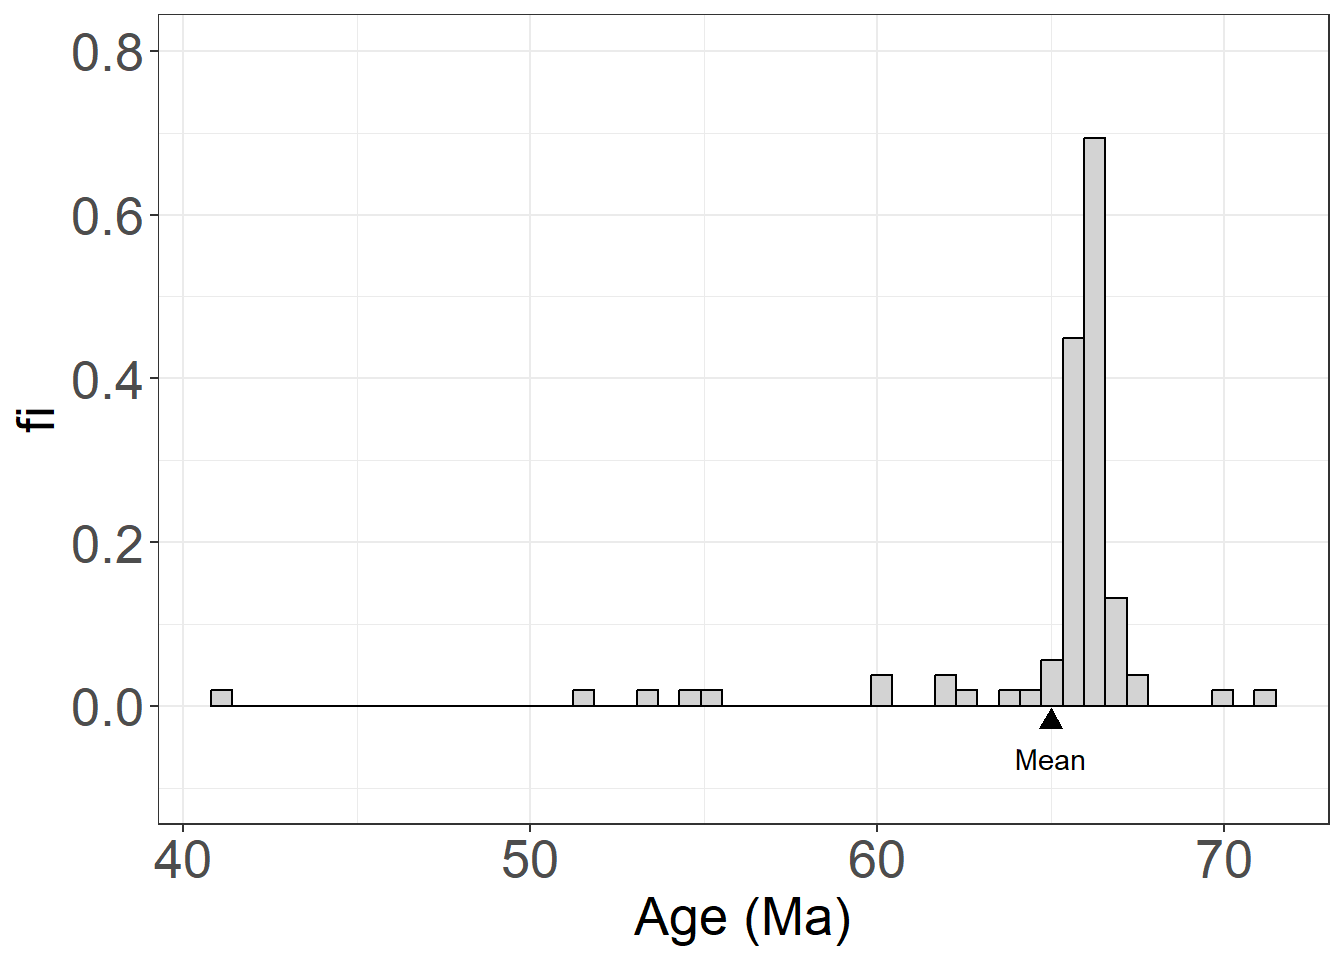
\includegraphics{_main_files/figure-latex/unnamed-chunk-25-1.pdf}

\hypertarget{questions}{%
\section{Questions}\label{questions}}

\textbf{1)} In the following boxplot, the first quartile and second quartile of the data are:

\textbf{\(\qquad\)a:} \((-1.00, 21.30)\); \textbf{\(\qquad\)b:} \((-1.00, 7.02)\); \textbf{\(\qquad\)c:} \((7.02, 7.96)\); \textbf{\(\qquad\)d:} \((7.02, 14.22)\)

\textbf{2)} The main disadvantage of a histogram is that:

\textbf{\(\qquad\) a :} Depends on the size of the bin ; \textbf{\(\qquad\)b :} Cannot be used for categorical variables;

\textbf{\(\qquad\) c :} Cannot be used when the bin size is small;
\textbf{\(\qquad\) d :} Used only for relative frequencies;

\textbf{3)} If the relative cumulative frequencies of a random experiment with outcomes \(\{1,2,3,4\}\) are: \(F(1)=0.15, \qquad F(2)=0.60, \qquad F(3)=0.85, \qquad F(4)=1\).

Then the relative frequency for the outcome \(3\) is

\textbf{\(\qquad\)a:} \(0.15\); \textbf{\(\qquad\)b:} \(0.85\); \textbf{\(\qquad\)c:} \(0.45\); \textbf{\(\qquad\)d:} \(0.25\)

\textbf{4)} In a sample of size \(10\) from a random experiment we obtained the following data:

\(8, \qquad 3, \qquad 3, \qquad 7, \qquad 3, \qquad 6, \qquad 5, \qquad 10, \qquad 3, \qquad 8\).

The first quartile of the data is:

\textbf{\(\qquad\)a:} \(3.5\); \textbf{\(\qquad\)b:} \(4\); \textbf{\(\qquad\)c:} \(5\); \textbf{\(\qquad\)d:} \(3\)

\textbf{5)} Imagine that we collect data for two quantities that are not mutually exclusive, for example, the gender and nationality of passengers on a flight. If we want to make a single pie chart for the data, which of these statements is true?

\textbf{\(\qquad\)a :} We can \textbf{only} make a nationality pie chart because it has more than two possible outcomes;

\textbf{\(\qquad\)b :} We can make a pie graph for a new variable marking gender \textbf{and} nationality;

\textbf{\(\qquad\)c :} We can make a pie chart for the variable sex \textbf{or} the variable nationality;

\textbf{\(\qquad\)d :} We can only choose \textbf{whether} to make a pie chart for gender \textbf{or} a pie chart for nationality.

\hypertarget{exercises}{%
\section{Exercises}\label{exercises}}

\hypertarget{exercise-1}{%
\subsubsection{Exercise 1}\label{exercise-1}}

We have performed an experiment 8 times with the following results

\begin{verbatim}
## [1]  3  3 10  2  6 11  5  4
\end{verbatim}

Answer the following questions:

\begin{itemize}
\tightlist
\item
  Calculate the relative frequencies of each result.
\item
  Calculate the cumulative frequencies of each result.
\item
  What is the average of the observations?
\item
  What is the median?
\item
  What is the third quartile?
\item
  What is the first quartile?
\end{itemize}

\hypertarget{exercise-2}{%
\subsubsection{Exercise 2}\label{exercise-2}}

We have performed an experiment 10 times with the following results

\begin{verbatim}
##  [1] 2.875775 7.883051 4.089769 8.830174 9.404673 0.455565 5.281055 8.924190
##  [9] 5.514350 4.566147
\end{verbatim}

Consider 10 bins of size 1: {[}0,1{]}, (1,2{]} \ldots( 9,10).

Answer the following questions:

\begin{itemize}
\item
  Calculate the relative frequencies of each result and draw the histogram
\item
  Calculate the cumulative frequencies of each result and draw the cumulative graph.
\item
  Draw a box plot .
\end{itemize}

  \bibliography{book.bib,packages.bib}

\end{document}
